\section{Mục tiêu bài Lab 2}
Mục tiêu của Lab 2 nhằm giúp sinh viên:
\begin{itemize}
    \item Hiểu cách biểu diễn bài toán Reinforcement Learning bằng Q-table.
    \item Nắm vững cơ chế $\epsilon$-greedy exploration để cân bằng giữa khám phá và khai thác.
    \item Phân biệt giữa thuật toán On-policy (SARSA) và Off-policy (Q-learning).
    \item Hiểu bản chất của Temporal Difference (TD) Learning.
\end{itemize}

\section{Thiết lập môi trường và thuật toán}
\subsection{Môi trường FrozenLake-v1}
Bài toán yêu cầu Agent tìm đường từ ô START (S) đến ô GOAL (G) trên một hồ băng.
\begin{itemize}
    \item \textbf{State space:} 16 trạng thái (4x4).
    \item \textbf{Action space:} 4 hành động (0: Left, 1: Down, 2: Right, 3: Up).
    \item \textbf{Reward:} +1 khi đến đích, 0 cho các trạng thái khác.
    \item \textbf{Tính chất:} Môi trường có tính ngẫu nhiên khi \texttt{is\_slippery=True}, hành động của Agent có thể dẫn đến kết quả không mong muốn.
\end{itemize}

\subsection{Cài đặt thuật toán}
\textbf{a. Q-Learning (Off-policy):}
Cập nhật giá trị Q dựa trên hành động tối ưu giả định ở trạng thái kế tiếp:
\begin{equation}
    Q(s, a) \leftarrow Q(s, a) + \alpha [r + \gamma \max_{a'} Q(s', a') - Q(s, a)]
\end{equation}

\textbf{b. SARSA (On-policy):}
Cập nhật giá trị Q dựa trên hành động thực tế $a'$ sẽ thực hiện ở trạng thái kế tiếp theo chính sách hiện tại:
\begin{equation}
    Q(s, a) \leftarrow Q(s, a) + \alpha [r + \gamma Q(s', a') - Q(s, a)]
\end{equation}

\section{Kết quả thực nghiệm và Phân tích}
Trong thí nghiệm này, cả hai thuật toán được huấn luyện trong 80,000 episodes với các siêu tham số: $\alpha = 0.1$, $\gamma = 0.99$, $\epsilon$ giảm dần từ 1.0 về 0.001.

\begin{figure}[H]
    \centering
    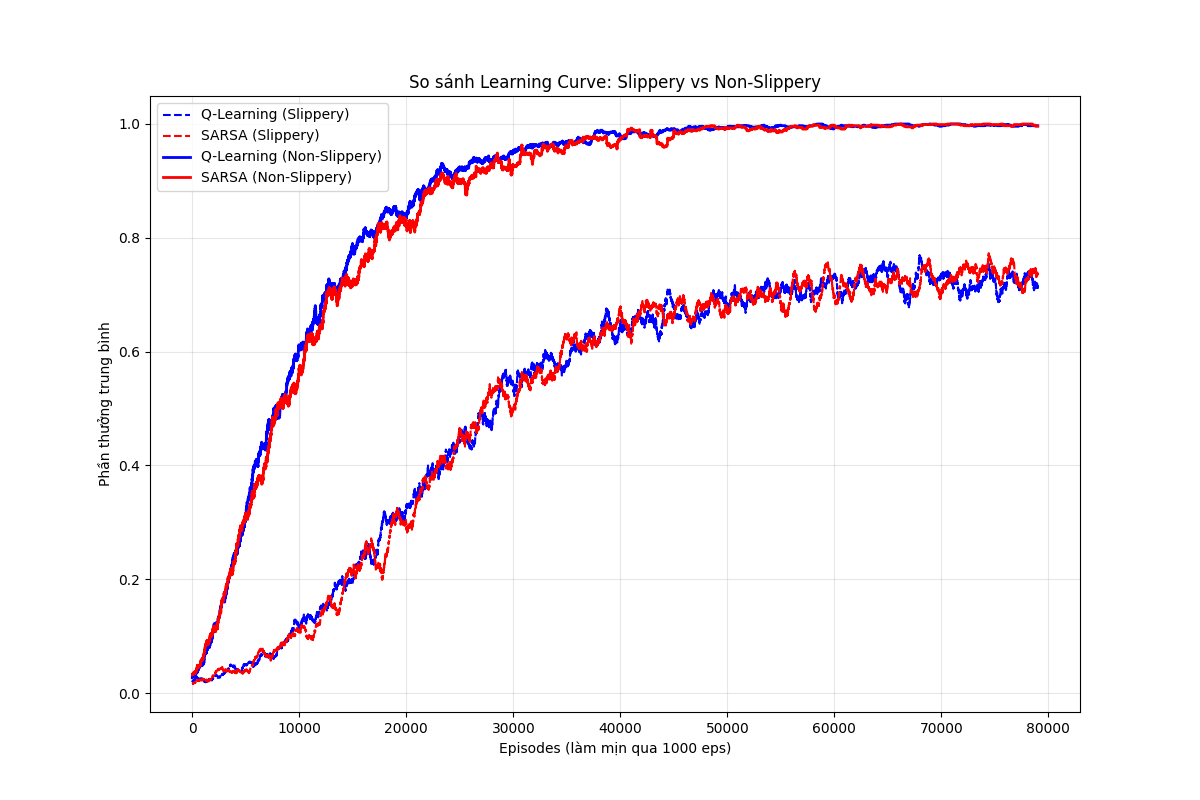
\includegraphics[width=0.9\textwidth]{Images/Lab2/comparison_slippery.png}
    \caption{So sánh Learning Curve: Q-Learning vs SARSA (Slippery và Non-Slippery)}
    \label{fig:comparison_lab2}
\end{figure}

\textbf{Phân tích đồ thị:}
\begin{itemize}
    \item \textbf{Môi trường Non-Slippery (Dễ):} Cả Q-learning và SARSA đều hội tụ rất nhanh về mức Reward $\approx 1.0$ (tỉ lệ thắng gần 100\%). Điều này dễ hiểu vì không có yếu tố ngẫu nhiên, Agent chỉ cần tìm được đường ngắn nhất.
    \item \textbf{Môi trường Slippery (Khó):} Tốc độ hội tụ chậm hơn đáng kể. Cả hai thuật toán đạt mức Reward ổn định khoảng $0.72 - 0.74$. 
    \item \textbf{So sánh Q-learning và SARSA:} Trong môi trường FrozenLake cơ bản này, sự khác biệt về Reward cuối cùng giữa hai thuật toán là không quá lớn. Tuy nhiên, SARSA thường có xu hướng ổn định hơn trong giai đoạn đầu huấn luyện vì nó tính đến cả rủi ro của các hành động khám phá ngẫu nhiên.
\end{itemize}

\section{Trả lời câu hỏi lý thuyết}

\subsection{Câu 1: Nguyên lý Q-learning và tính Off-policy}
Q-learning học hàm giá trị $Q(s, a)$ bằng cách sử dụng sai số Temporal Difference. Nó được gọi là \textbf{Off-policy} vì quy tắc cập nhật của nó sử dụng giá trị của hành động tốt nhất có thể ($\max Q(s', a')$) để ước lượng phần thưởng tương lai, bất kể hành động thực tế mà Agent thực hiện ở bước tiếp theo là gì (có thể là một hành động ngẫu nhiên do $\epsilon$-greedy).

\subsection{Câu 2: So sánh Q-learning và SARSA}
Sự khác biệt nằm ở thành phần mục tiêu (target) trong công thức cập nhật:
\begin{itemize}
    \item \textbf{Q-learning:} Dùng $\max_{a'} Q(s', a')$ - giả định Agent luôn chọn hành động tốt nhất. Điều này giúp nó tìm ra đường đi tối ưu nhanh hơn nhưng có thể mạo hiểm.
    \item \textbf{SARSA:} Dùng $Q(s', a')$ - với $a'$ là hành động thực tế được chọn bởi chính sách hiện tại. Điều này làm SARSA trở nên "thận trọng" hơn vì nó học được rằng các hành động khám phá có thể dẫn đến kết quả xấu (rơi vào hố).
\end{itemize}

\subsection{Câu 3: Vai trò của chính sách $\epsilon$-greedy}
Chính sách này giúp cân bằng giữa \textbf{Exploration} (Khám phá môi trường mới) và \textbf{Exploitation} (Khai thác kiến thức đã học).
\begin{itemize}
    \item \textbf{Nếu $\epsilon$ quá lớn:} Agent liên tục chọn hành động ngẫu nhiên, dẫn đến việc không bao giờ hội tụ về chính sách tối ưu.
    \item \textbf{Nếu $\epsilon$ quá nhỏ:} Agent ít khám phá, dễ bị kẹt vào các cực trị địa phương (local optima) và không tìm thấy đường đi tốt nhất nếu nó chưa từng đi qua.
\end{itemize}

\subsection{Câu 4: Thuật toán nào an toàn hơn?}
Trong môi trường có tính rủi ro cao, \textbf{SARSA học an toàn hơn}. Vì SARSA là on-policy, nó cập nhật Q-value dựa trên hành động thực tế (bao gồm cả các bước đi ngẫu nhiên). Nếu một đường đi tối ưu nằm ngay sát các hố nguy hiểm, SARSA sẽ nhận thấy rủi ro rơi vào hố khi khám phá và sẽ chọn một đường đi xa hơn nhưng an toàn hơn. Q-learning phớt lờ rủi ro này vì nó luôn giả định sẽ đi tối ưu ở bước sau.

\subsection{Câu 5: Nguyên nhân đồ thị Reward không ổn định}
Ba nguyên nhân phổ biến và cách khắc phục:
\begin{enumerate}
    \item \textbf{Learning rate ($\alpha$) quá lớn:} Khiến giá trị Q dao động mạnh và không hội tụ. \textit{Khắc phục:} Giảm $\alpha$ theo thời gian.
    \item \textbf{$\epsilon$ decay quá chậm:} Agent dành quá nhiều thời gian để khám phá ngẫu nhiên ngay cả khi đã học được chính sách tốt. \textit{Khắc phục:} Tăng tốc độ giảm $\epsilon$.
    \item \textbf{Reward quá thưa thớt (Sparse Reward):} Agent hiếm khi chạm tới đích nên không có đủ tín hiệu để cập nhật. \textit{Khắc phục:} Tăng số lượng episodes hoặc thực hiện Reward Shaping.
\end{enumerate}
